\documentclass[11pt]{article}

\usepackage{fourier}
\usepackage[T1]{fontenc}
\usepackage[top=1in, bottom=1in, left=1in, right=1in]{geometry}
\usepackage[usenames, dvipsnames, svgnames]{xcolor}
\usepackage{enumitem}
\usepackage{titling}
\usepackage[small, compact]{titlesec}
\setitemize[0]{leftmargin=*}
\usepackage{amsfonts, amsmath, amssymb}
\usepackage{multicol, multirow}
\usepackage{epsfig, subfigure, subfloat, graphicx}
\usepackage{anysize, indentfirst, setspace}
\usepackage{verbatim, rotating, xfrac}
\usepackage{gensymb}
\usepackage{caption, hanging}
\newcommand{\mc}[1]{\multicolumn{1}{c}{#1}}
%\parindent 0pt
%\setdefaultenum{a.}{i.}{A}{1}
%\setdefaultitem{}{\textperiodcentered}{}{}
\usepackage{booktabs}
\usepackage{dcolumn}
\usepackage{caption, hanging}
\usepackage{tikz}
\usetikzlibrary{shapes,arrows,backgrounds}
%\setdefaultenum{a.}{1)}{i.}{a.}
\parindent 0pt

\makeatletter
\newcommand{\distas}[1]{\mathbin{\overset{#1}{\kern\z@\sim}}}%
\newsavebox{\mybox}\newsavebox{\mysim}
\newcommand{\distras}[1]{%
  \savebox{\mybox}{\hbox{\kern3pt$\scriptstyle#1$\kern3pt}}%
  \savebox{\mysim}{\hbox{$\sim$}}%
  \mathbin{\overset{#1}{\kern\z@\resizebox{\wd\mybox}{\ht\mysim}{$\sim$}}}%
}
\makeatother

\title{\Large{\bf{\vspace{-100pt}Mathematics for Political Science \vspace{-15pt}}}}
\author{\large{Exercise 1: Foundations \& Algebra}}
\date{August 17\textsuperscript{th}, 2020}
\begin{document}
\maketitle

\hrule

\begin{enumerate}

\item For the coffeeshop data from lecture, classify each quantitative variable as:
\begin{enumerate}
\item dichotomous, discrete, or continuous
\item categorical, ordinal, interval, or ratio
\end{enumerate}


\item Using the data in the table below:
\begin{enumerate}
		\item Find output for the functions $f(x)$ and $g(x)$.
		\item Show the functions equivalent to $f(g(x))$ and $g(f(x))$.
		%f(g(x)) = (7-2x^3)^2 = 49-28x^3 + 4x^6, g(f(x))=2(3-x)^6-4
		\item Find the output for these functions.
\end{enumerate}

\begin{small}
\begin{center}
\begin{tabular}{c|c|c|c|c}
x & $f(x) = (3-x)^2$  & $g(x) = 2x^3 - 4$   & $f(g(x))$  & $g(f(x))$\\ \hline
2 &                   &                     &            &           \\
4 &                   &                     &            &           \\
5 &                   &                     &            &           \\
1 &                   &                     &            &           \\
0 &                   &                     &            &           \\
1 &                   &                     &            &           \\
\end{tabular}
\end{center}
\end{small}


\item Express each of the following complex functions as two simpler functions, one nested inside the other:
\begin{enumerate}
		\item $4(8x-2)^3$ %g(x) = 8x-2, f(x) = 4x^3
		\item $\frac{1}{3x-2}$ %g(x)=3x-2, f(x) = 1/x
\end{enumerate}


\item Explain why there is no ``largest number'' on the interval $(0,1)$.


\item Plot (roughly) the following functions in coordinate space (use separate graphs):
\begin{enumerate}
\item $f(x) = 2x^2$ for $x \in [0,10]$
\item $f(x) = e^{x}$ for $x \in [0,4]$
\item $f(x) = \frac{1}{x}$ for $x \in (0,\infty)$
\item $f(x) = x^3 - x^2 + 1$ for $x \in [0,1]$
\item $f(x)=\left\{\begin{array}{cl}
	-(x^2)  & \textrm{~for~} x \in [-2,0)\\
	\frac{1}{2} & \textrm{~for~} x = 0\\
    x^3 + 1 & \textrm{~for~} x \in (0,2]\\
	   \end{array}\right.$
\end{enumerate}



\item (Gill 1.14 [adapted]) The following data are U.S. Census Bureau estimates of population over a 5 year period.

\begin{center}
\begin{tabular}{lr}
Date         & Total U.S. Population \\ \hline
July 1, 2004 & 293,655,404 \\
July 1, 2003 & 290,788,976 \\
July 1, 2002 & 287,941,220 \\
July 1, 2001 & 285,102,075 \\
July 1, 2000 & 282,192,162 \\ \hline
\end{tabular}
\end{center}

Characterize the growth in terms of an approximate parametric expression.  Graphing may help (optional).
% p \approx 282,200,000 + 2,800,000*y


\item Explain in words the difference between a concave and convex function.  Draw one of each to illustrate. 
% conCAVE looks like a cave entrance, conVex looks like a V


\item Characterize the functions below as monotonic or non-monotonic.

\begin{center}
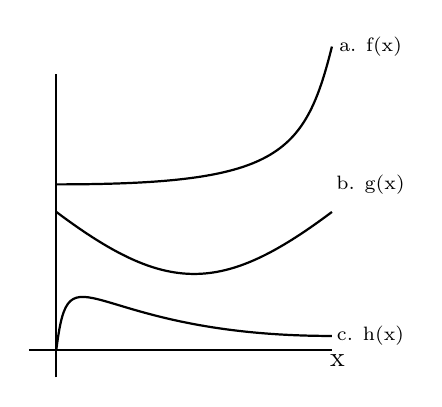
\begin{tikzpicture}[scale=.7]
\draw[thick] (-.5,0) -- (5,0);
\draw[thick] (0,-.5) -- (0,5);
\draw (5.1,-0.2) node{x};
\draw[thick] (0,0) .. controls (.25,2) and (.5,.25) .. (5,.25);
\draw (5.7,.25) node{\scriptsize{c. h(x)}};
\draw[thick] (0,2.5) .. controls (2,1) and (3,1) .. (5,2.5);
\draw (5.7,3) node{\scriptsize{b. g(x)}};
\draw[thick] (0,3) .. controls (4,3) and (4.5,3.5) .. (5,5.5);
\draw (5.7,5.5) node{\scriptsize{a. f(x)}};
\end{tikzpicture}
\end{center}
% a monotonic, b and c not


\item Given the data below, find:
\begin{enumerate}
\item $\displaystyle\sum_1^{10} \frac{m_i}{2}$ %39/2
\item $\displaystyle\prod_1^{6} (m_i - 5$) %-6
\end{enumerate}
\begin{center}
\begin{tabular}{c|c|c|c|c|c|c|c|c|c}
$m_1$  & $m_2$ & $m_3$ & $m_4$ & $m_5$ & $m_6$ & $m_7$ & $m_8$ & $m_9$ & $m_{10}$   \\ \hline
3      & 1     & 8     & 3     & 2     & 7     & 4     & 5     & 4     & 2       \end{tabular}
\end{center}



\item (Gill 1.1 [adapted]) Simplify the following expressions as much as possible (if any simplification is possible):
\begin{center}
\begin{tabular}{p{3cm}p{3cm}p{3cm}}
a. $(-x^4y^2)^2$       &  b. $9(3^0)$                                 & c. $(2a^2)(4a^4)$                     \rule{0cm}{1cm}\\
d. $\displaystyle\frac{x^4}{x^3}$   &  e. $y^3 + y^4 + y^5$                        & f. $\displaystyle\frac{\frac{2a}{7b}}{\frac{11b}{5a}}$ \rule{0cm}{1cm}\\
g. $\ln (\frac{e^4}{3})$& h. $\displaystyle\log_8 1$
\rule{0cm}{1cm}\\
\end{tabular}
\end{center}


\item (Gill 1.2 [adapted]) Simplify the following expressions by expanding the polynomials and grouping like terms:
\begin{enumerate}
		\item $(a+b)^2 + (a-b)^2 + 2(a+b)(a-b) - 3a^2$ %a^2
		\item $3p(q+p)^2 - pq + 4x(q + 2p)^2$ %3pq^2 + 6p^2 q + 3p^3 - pq + x(4q^2 + 16pq +16p^2)
\end{enumerate}


\item Suppose the vote totals a candidate will receive are given by the equation:
\begin{equation*}
V = b + 8s^{\frac{1}{2}}
\end{equation*}
Where $V$ is the number of votes, $b$ is the candidate's number of baseline loyal supports, and $s$ is the amount of money they spend on the campaign.
\begin{enumerate}
\item If candidate A has loyalists $b_A = 20,000$ and spends $s_A = \$1,000,000$, and candidate B has loyalists $b_B = 25,000$ and spends $s_B = \$250,000$, which one will win the election? %B wins 29,000 to 28,000
\item Approximately how would the losing candidate have had to spend to pull even?  How much additional spending is that? % total of 1,265,625, or 265,625 more
\end{enumerate}


\item (Gill 1.12) Suppose we are trying to put together a Congressional committee that has representation from four national regions.  Potential members are drawn from a pool with 7 from the northeast, 6 from the south, 4 from the Midwest, and 6 from the far west.  How many ways can you choose a committee that has 3 members from each region for a total of 12?\\ % 56,000





% ----------------------------------------------------
%   algebra
% ----------------------------------------------------
\item Solve the following equations for x:
\begin{enumerate}
\item $12x + 2 = 18x$ %x = 1/3
\item $-6 - 4x = -3 - 8x$  %x = 3/4
\end{enumerate}


\item Express $\alpha$ in terms of the other unknown variables:
\begin{enumerate}
\item $3\alpha - 8\theta = \alpha + 2\beta$ %alpha = beta + 4 theta
\item $\alpha x + \alpha y = \alpha x^2 + \alpha y^2 + 4$ %alpha = 4/(x + y - x^2 - y^2)
\end{enumerate}


\item (Gill 1.6) Solve the following inequalities so that the variable is the only term on the left-hand side:
\begin{enumerate}
\item $x - 3 < 2x + 15$  %x > -18
\item $11 - \frac{4}{3}t > 3$  % t < 6
\item $\frac{5}{6}y + 3(y-1) \leq \frac{11}{6}(1-y) + 2y$  % y \leq 29/22
\end{enumerate}


\item Find the values of $x$ where $f(x)=0$ using factorization:
\begin{enumerate}
\item $x^2 + 5x - 14$ % x=2, x=-7 (x-2)(x+7)
\item $x^2 - 8x + 16$ % x=4 (x-4)^2
\item $3x^2 + 9x - 30$ % x=2, x=-5 (3x-6)(x+5)
\end{enumerate}


\item Solve the following equations for $x$ using the quadratic formula:
\begin{enumerate}
\item $18x^2 + 10x = 3 - 15x$ %x=1/9, x=-1.5
\item $20x^2 + 2x - 3 = 5 + 20x - 15x^2$ % x= -2/7, x=4/5
\end{enumerate}


\item Solve the following systems of equations for $a$ and $b$ using the ``direct substitution'' approach:
\begin{enumerate}
\item $b + 5a = 2$ \\ $7b - 6a = 14$ %a=0, b=2
\item $3(a+b) + 7a = 8(b-1) + 33$ \\ $-3a + 4(1-b) = 4(1-a) - 15$ %a=5, b=5
\end{enumerate}



\item Solve the following systems of equations for $c$ and $d$ using the ``elimination'' approach:
\begin{enumerate}
\item $3c + 4d = 13$ \\ $2c + 5d = 4$ %c=7, d=-2
\item $c + 4d + 36 = 10d - 3c$ \\ $2(c+1) + 2(d+1) = 6$ %c=-3, d=4
\end{enumerate}


\item Solve this system of equations for $x$ and $y$ in terms of $\alpha$: \\
$~~~~~~~~2x + y = 10\alpha + 5$ \\
$~~~~~~~~3x + 3y = 18\alpha + 9$ % x=4a + 2, y=2a + 1


\item Solve this system of equations for q, r, and s: \\
$~~~~~~~~2q + 4r + s = 1$ \\
$~~~~~~~~4(q+1) + 7(1-r) = 2s + 16$ \\
$~~~~~~~~8q + 4r - 2s = 5q + 19r + 4s$ % q=1, r=-1, s=3


\item Calculate the dot product of the vectors below.
\begin{enumerate}
\item $[3, 4, 1, 7, 0] \cdot [5, 2, 2, 0, 3]$ %25
\item $[4, 1, 3] \cdot [0, 7, 5]$ %22
\end{enumerate}



\item (Gill 3.9) For the following matrix, calculate $\textbf{X}^n$ for $n = 2, 3, 4, 5$.  Write a rule for calculating higher values of $n$.
\[
\left[\begin{array}{ccc}
0 & 0 & 1 \\
0 & 1 & 0 \\
1 & 0 & 0 \\
\end{array}\right]
\]
% odd powers look like this, even powers are the identity matrix


\item Using the matrix below, show the identities of multiplication and addition for matrices:
\[
\left[\begin{array}{cc}
a & b \\
c & d \\
\end{array}\right]
\]



\item Perform the following matrix multiplications, or explain why they are not possible:
\begin{enumerate}
\item $\left[\begin{array}{cccc}
4 & 5 & 5 & 2 \\
\end{array}\right]
\left[\begin{array}{cc}
1 & 3 \\
8 & 1 \\
0 & 9 \\
6 & 4 \\
\end{array}\right]$
% [56  70]
\item $\left[\begin{array}{ccc}
a & b & c \\
d & e & f \\
g & h & i \\
\end{array}\right]
\left[\begin{array}{c}
p \\
q \\
r \\
\end{array}\right]$
\item $\left[\begin{array}{ccc}
\alpha & \beta    & \gamma \\
\delta & \epsilon & \eta \\
\end{array}\right]
\left[\begin{array}{cc}
\lambda & \sigma \\
\end{array}\right]$
% not possible - doesn't conform
\end{enumerate}




\item Multiply the matrices below to show that order matters for matrix multiplication: 

\begin{tabular}{cccc}
&
a. $\left[\begin{array}{ccc}
4 & 7 & 1 \\
\end{array}\right]
\left[\begin{array}{c}
3 \\
0 \\
5 \\
\end{array}\right]$
&
~~~~~~~~
&
$\left[\begin{array}{c}
3 \\
0 \\
5 \\
\end{array}\right]
\left[\begin{array}{ccc}
4 & 7 & 1 \\
\end{array}\right]$
\end{tabular}


\begin{tabular}{cccc}
&
b. $\left[\begin{array}{cc}
4 & 8 \\
1 & 6 \\
2 & 2 \\
\end{array}\right]
\left[\begin{array}{ccc}
9 & 6 & 3 \\
1 & 5 & 3 \\
\end{array}\right]$
&
~~~~~~~~
&
$\left[\begin{array}{ccc}
9 & 6 & 3 \\
1 & 5 & 3 \\
\end{array}\right]
\left[\begin{array}{cc}
4 & 8 \\
1 & 6 \\
2 & 2 \\
\end{array}\right]$
\end{tabular}




\end{enumerate}



\vfill
\begin{center}
\small{Thanks to Sarah Bouchat, Michael DeCrescenzo, Brad Jones, and Dave Ohls for past years' materials.}
\end{center}

\end{document} 